\phantomsection
\addcontentsline{toc}{chapter}{Appendices}

% The \appendix command resets the chapter counter, and changes the chapter numbering scheme to capital letters.
%\chapter{Appendices}
\appendix
\chapter{Machine Learning}
\label{app:ml}

\section{Vanishing Gradient}
\label{app:ml:van_grad}
When training neural network using back-propagation, each of the network layer's weights receives an update by computing a partial derivative given its next layer's partial derivative using chain rule. The problem is the weights of the layer can be small i.e. (0, 1], this is especially the case if you use a traditional activation such as hyperbolic tangent function which clips the output to range of (0, 1]. When back-propagating, the gradient is going to be multiplied by a value in range of (0,1] many times. This means that the gradient is getting smaller and smaller as we back-propagate (thus the term \textit{vanishing}), and when it finally reaches beginning layers of the network, the gradient can be too small for them to perform any meaningful update, thus preventing the layers from learning. For a deep network such as GAN, vanishing gradient is more likely to occur since the gradient need to be back-propagated through both discriminator and generator. A closely related problem is exploding gradient problem, which the gradient increases instead of decreases. There have been multiple proposed solutions to this problem. I will briefly describe them below:

\begin{itemize}
    \item \textbf{Batch Normalization} is a widely adopted method for solving both exploding and vanishing gradient problem. It reduces the internal covariate shift\cite{ioffeBatchNormalizationAccelerating2015a} and reduces local optimum by smoothing the optimization landscape\cite{santurkarHowDoesBatch2018}.
    \item \textbf{Residual Network} is the most effective way to solve the vanishing gradient problem. It refers to a network architecture that implements skip/residual connection. It creates shortcuts for gradient to flow through without diminishing/exploding.
    \item \textbf{Activation Function} if used appropriately, can reduce the chance of vanishing gradient. For example, ReLU suffers less because gradient does not saturate on the active path (i.e. positive values)\cite{glorotDeepSparseRectifier2011}.
    \item \textbf{Weight Initialization}\label{app:ml:van_grad:weight_init} could be helpful to reduce weight initialization by adjusting them to follow a certain distribution. For example, Xavier\cite{glorotUnderstandingDifficultyTraining2010} initialize weights such that mean of the activations are zeros, and the variance of the activations stay the same across every layer. In other words, weights of a layer $l$ are randomly sampled from a Gaussian/normal distribution with mean $\mu = 0$ and variance $\sigma^2=\frac{1}{n_{l-1}}$, where $n_{l-1}$ is the number of neurons in the previous layer, and bias are initialized with zeros.
\end{itemize}

\section{Mode Collapse}
\label{app:ml:mode_col}
A well trained model would produce a wide variety of outputs, however, it may stuck in a special kind of local minimum. Let's consider a scenario: our generator found a small subset of outputs that produces an especially plausible for the discriminator, we call the current version of generator $\mathcal{G}_1$ and discriminator $\mathcal{D}_1$. As training continues, the discriminator would learn to reject this subset and result in $\mathcal{D}_2$.  However, the generator evolves to $\mathcal{G}_2$ as well and learned to produce another small subset of plausible output for $\mathcal{D}_2$. Now in order to learn to reject $\mathcal{G}_2$'s output, the discriminator may not evolves to a new $\mathcal{D}_3$, instead, it may fallback to $\mathcal{D}_1$, because it can probably reject $\mathcal{G}_2$'s output as well. Then the generator and discriminator just cycling through these two versions and not making any real progress. This form of failure is called mode collapse.

\section{Non-Convergence}
\label{app:ml:non_conv}
As the generator improves over time, the discriminator performance will get worse, because it can no longer tell a difference between real and fake output. The discriminator will just make random guess. Now the feedback from the discriminator is meaningless and can degrade generator performance, when the generator performance degrades, the discriminator can again provide meaningful feedback, and the loop continues. This means that when training GAN, it is hard to determine when to stop, as it does not necessarily reduced to a stable state.

\section{Symmetry Problem}
\label{app:ml:sym}
In the context of weight initialization, symmetry problem is an argument for weights should not be initialized as same value. This is because if the weights are equal, then its gradient will be equal, and the weights are going to be updated by the same amount. If these weights are attached to the same neuron, it will theoretically remain the same throughout training, and therefore its capability will decrease.

\section{Knowledge Distillation}
\label{app:ml:kd}
While large models such as very deep neural network can have large capacity, it may not be fully utilized. This means that we can potentially reduce the size of the model while achieve similar results. This process is called knowledge distillation.

\section{Weight Clipping}
\label{app:ml:weight_clip}
Weight clipping is to enforce gradient in a network to have a specific minimum or/and maximum if they exceed a certain range. It can be used to prevent exploding gradient, but generally this does not fix the real underlying problem. More commonly, it is used in Wasserstein GAN to enforce the \textit{dual representation theorem} constraint so that Wasserstein distance can be computed efficiently. Let $W$ be any $m\times l$ matrix, $c=\max|W|$, and $||\cdot||_s$ be operator norm of the matrix (the element with largest singular value, in other words, the maximum absolute value of its eigenvalues), we have:
$$
||W||_s^2\leq c^2ml^2
$$
by clipping all entries of $W$ within some interval $[-c, c]$. Thus we can bound $||W||_s$ and restricted the discriminator to have bounded Lipschitz norm.

\section{Gradient Penalty}
\label{app:ml:grad_pen}
Gradient penalty is used in Wasserstein GAN to enforce the \textit{dual representation theorem} constraint so that Wasserstein distance can be computed efficiently. It is a loss for the discriminator in GAN in the form of:
$$
\mathbb{E}_{x \sim \hat{\mu}}\left[\left(\|\nabla D(x)\|_{2}-a\right)^{2}\right]
$$
where $\hat{\mu}$ is a fixed distribution, and $a$ is the targeted value. During training, the discriminator will attempt to minimize the difference between $\nabla D(x)$ and $a$, bringing all its gradient close to $a$, and thus restricts the discriminator to have bounded Lipschitz norm.

\section{Skip/Residual Connection}
\label{app:ml:res_conn}
Residual connection is a technique used to allow an neural network block to \textit{modify} the  input instead of \textit{transform} the input. Additionally, the output holds a reference to the input which allow gradient to shortcut the previous block directly. There is empirical evidence showing deep neural network built with this technique is easier to optimize. Essentially, applying such technique is to change a function $f$ from $f(x)$ to $f(x)+x$. Figure \ref{fig:res_conn} further illustrate such technique.

\begin{figure}
    \centering
    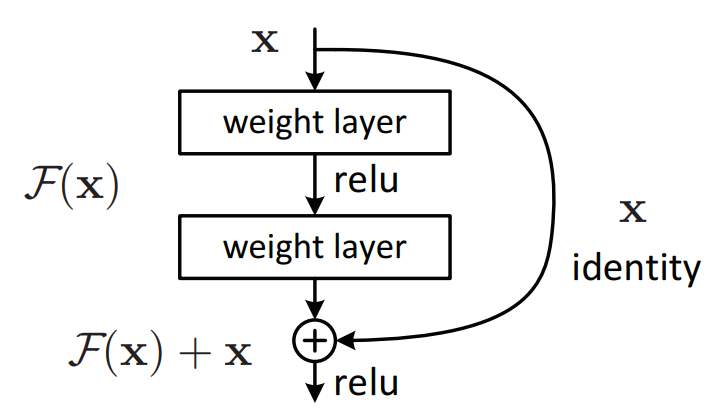
\includegraphics[width=0.45\textwidth]{images/preliminary/res_conn.png}
    \caption{Residual Connection block. The input of the block is element-wise added to the output of the block, creating shortcut for gradient to flow through.\cite{heDeepResidualLearning2015a}}
    \label{fig:res_conn}
\end{figure}

\section{Pre-Activation}
\label{app:ml:pre_act}

\section{Pixel Shuffle}
\label{app:ml:pix_shuf}

\begin{figure}
    \centering
    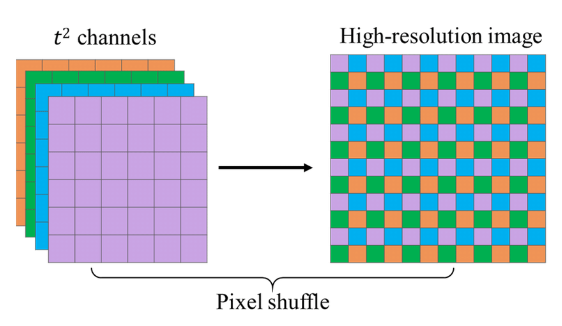
\includegraphics[width=0.45\textwidth]{images/appendix/pixel_shuffle.png}
    \caption{Illustration of the pixel shuffle operation. $t^2$ channels of features are combined in a interleaving manner, effectively result in a sub-pixel}
    \label{fig:pixel_shuffle}
\end{figure}

Pixels Shuffle is an function often used in super resolution model to implement efficient sub-pixel convolution. It convolute the image using $t^2$ channels and combine feature in different channels, interleaving each other. 

Note that this is a different operation than transpose convolution. Transpose convolution increases size of feature map by convolution with stride, while pixels shuffle increases resolution by flattening multiple feature maps into one. 



\chapter{Statistics}
\label{app:stat}

\section{tSNE}
\label{app:stat:tsne}
TSNE stands for t-distributed stochastic neighbor embedding. It is a probabilistic-based method for visualizing high dimensional data by assigning data points in different dimensions onto different regions on a 2 or 3 dimensional grid. Specifically, this assignment method is called Stochastic Neighbor Embedding\cite{hintonStochasticNeighborEmbedding2002}. A pleasant feature of this method is that it preserves neighbor identities, which means similar features will be placed closer together.

\section{ISOMAP}
\label{app:stat:isomap}


% \chapter{Another Appendix About Things}
% \label{appendixlabel2}
% (things)

% \chapter{Colophon}
% \label{appendixlabel3}
% \textit{This is a description of the tools you used to make your thesis. It helps people make future documents, reminds you, and looks good.}

% \textit{(example)} This document was set in the Times Roman typeface using \LaTeX\ and Bib\TeX , composed with a text editor. 
 % description of document, e.g. type faces, TeX used, TeXmaker, packages and things used for figures. Like a computational details section.
% e.g. http://tex.stackexchange.com/questions/63468/what-is-best-way-to-mention-that-a-document-has-been-typeset-with-tex#63503

% Side note:
%http://tex.stackexchange.com/questions/1319/showcase-of-beautiful-typography-done-in-tex-friends
